% https://userswww.pd.infn.it/~moretto/fontana/project/software/2018/03/16/compton-edge.html
\documentclass{article}
\usepackage[utf8]{inputenc}
\usepackage{blindtext}
\usepackage{graphicx}
\usepackage{amsmath}
\usepackage{csvsimple}
\usepackage{pdfpages}
\usepackage{hyperref}
\usepackage{gensymb}

\begin{document}
\begin{center}
\textbf{\Huge{University of South Bohemia}}\\
\vspace{50px}
\textbf{\Large{Faculty of Science}} \\
\vspace{30px}
\includegraphics[width=120px]{~/school/logo.png} \\
\vspace{30px}
\textbf{\large{Praktika IV}}
\vspace{20px}
\\
\vspace{20px}
\large{Relativistické chování elektronů} \\
\vspace{60px}
\end{center}
\begin{flushleft}
Datum: 20.2.2024 \\
Jmeno: Martin Skok \\
Obor: Fyzika \\
Hodnoceni:
\end{flushleft}
\newpage
\section{Úkoly}
\begin{itemize}
  \item Na HPGe detektoru proměřte spektra $\gamma$-záření připravených radioizotopů
  \item Určete energie peaků plného pohlcení a energie jím příslušejících Comptnových hran
  \item Vypočtěte hybnosti odražených Comptnovkých elektronů a na grafech ukažte,
        zda se chovají dle klasické teorie nebo podle teorie relativity
\end{itemize}
\section{Pomůcky}
Zdroj gamma záření LABKIT-SR-Cs137, detektor Osprey, program ProSpect, Radiagem
2000, podložka s úhloměrem, ocelový kůl
\section{Teorie}
Comptnův rozptyl je, když se srazí foton s volným elektronem. Tímto foton předá nehybnému elektronu část svojí energie. Můžou se stát dvě věci. Energie fotonu se plně pohltí eletronem, takže předá elektronu všechnu svojí energii a zmizí. Toto se projeví ve spektru jako peak s maximální energií gamma $E_{\gamma}$, což je vlastně energie fotonu.
Druhá věc, co se může stát je, že se foton odrazí o $180^{\degree}$ a elektron získá maximální hybnost. Toto se projeví ve spektru jako comptona hrana $T$, což je energie předaná elektronu.
Hybnost elektronu pak můžeme určit ze vztahu
\begin{equation}\label{eq:hyb}
  pc = 2E_{\gamma} - T
\end{equation}
\section{Postup měření}
Zapnul jsem počítač a program ProSpect.
Nastavil jsem následné parametry podle návodu.
Vzal jsem zářič a umístil ho na detektor.
Spustil jsem start.
Označil jsem pomocí myši začátek a konec fotopeaku.
Provedl jsem kalibraci.
Data jsem uložil a opakoval pro další zářiče.
\newpage
\section{Data}
Data jsem vynesl do grafu a určil peaky a jejich náležící comptnovy hrany.
Začátek a konec comptnovské hrany je v grafu označená vertikálními čárami.
První je vždy graf celého spektra a další dva nebo jeden jsou zazoomované sekce,
aby byly dobře vidět comptnovy hrany.
\begin{figure}[!h]
  \hspace*{-1em}
  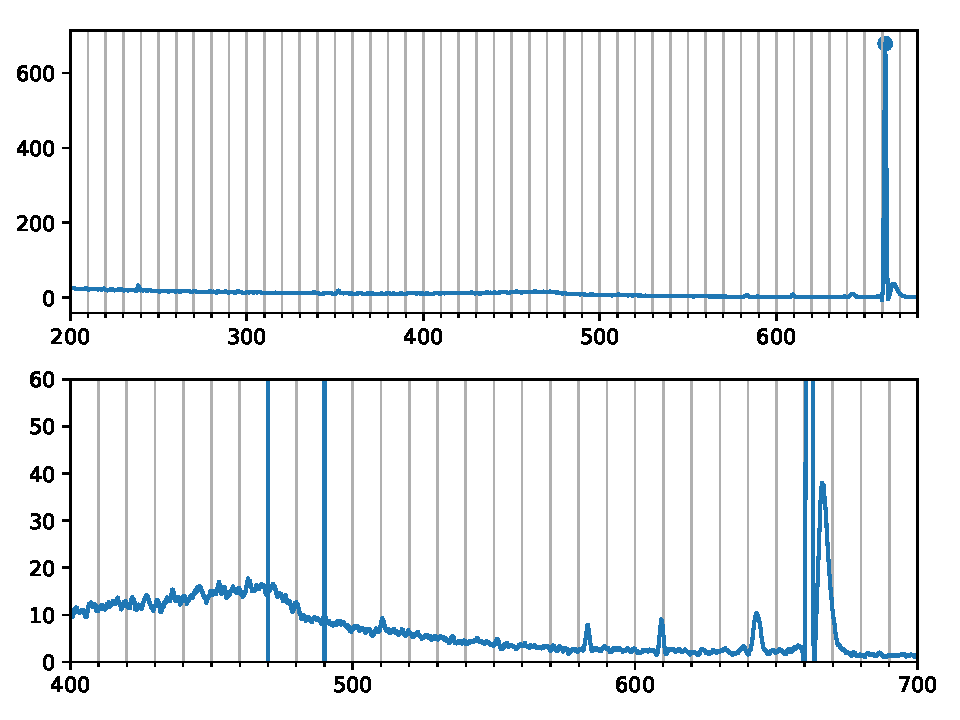
\includegraphics[scale=0.8]{figs/Cs137.pdf}
  \caption{Cs137}
\end{figure}
\newpage
\begin{figure}[!h]
  \hspace*{-1em}
  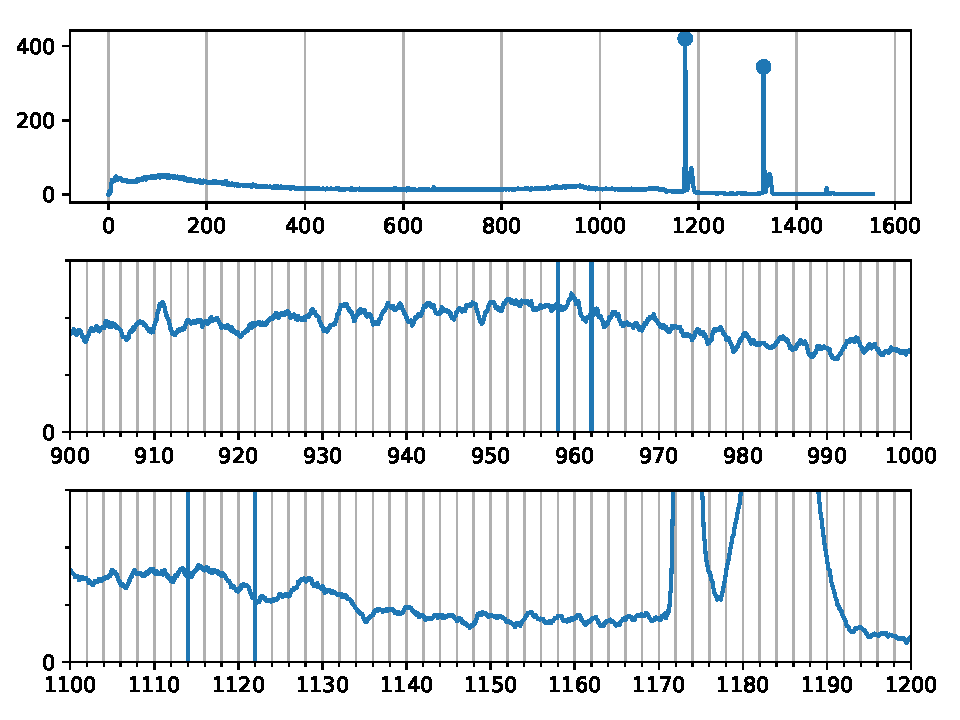
\includegraphics[scale=0.8]{figs/Co60.pdf}
  \caption{Co60}
\end{figure}
\newpage
\begin{figure}[!h]
  \hspace*{-1em}
  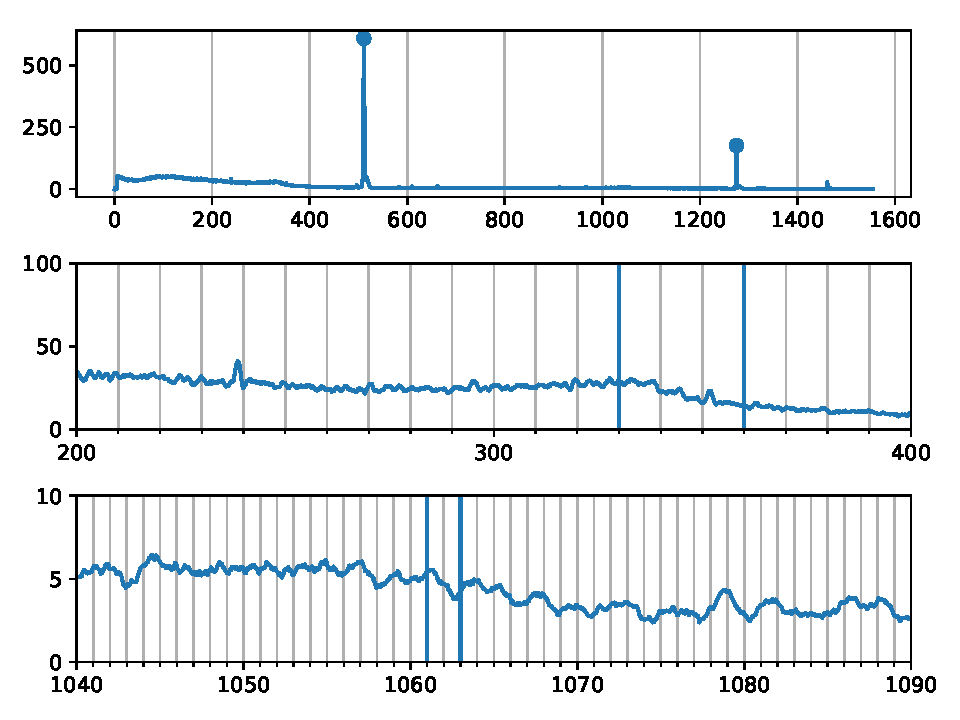
\includegraphics[scale=0.8]{figs/Na22.pdf}
  \caption{Na22}
\end{figure}
\newpage
\begin{figure}[!h]
  \hspace*{-1em}
  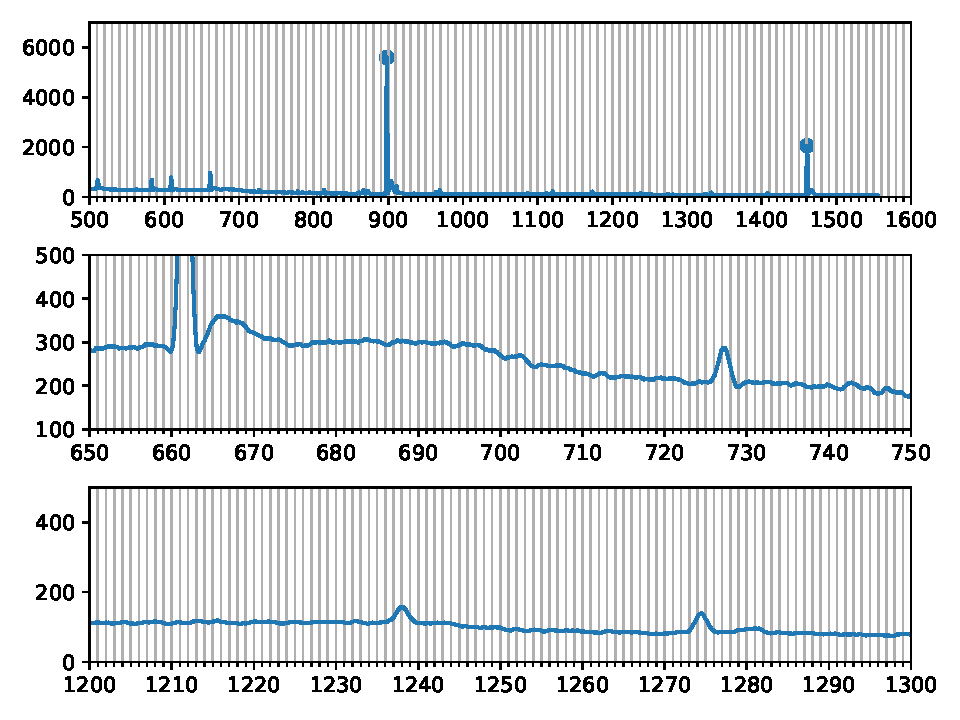
\includegraphics[scale=0.8]{figs/Y88.pdf}
  \caption{Y88}
\end{figure}
\newpage
\footnotesize{Tabulka 1:}\\
\\
\large{
\csvreader[
tabular = |c|c|c|c|c|c|,
table head =
\hline
{prvek}&{$E_{\gamma}$}&{comptnova}&{chyba comptnovy}&{hybnost}\\
{}&{(peaky)}&{hrana}&{hrany}&{eletronu}\\
\hline
\hline,
late after line = \\\hline
]{figs/df1.csv}{}{
  \csvcoli & \csvcolii & \csvcoliii & \csvcoliv & \csvcolv}
\\
}
\vspace{1em}
\\
Kde hybnost elektronu jsem spočítal podle vztahu \ref{eq:hyb}.\\
Chyba comptnovy hrany je střední odchylka dvou hodnot, a to začátku a konce comptnovy strany z grafu.
Potom jsem vynesl graf závislosti kinetické energie elektronu na jeho hybnosti.
Data jsem proložil křivkou klasické $T$ a relativistické $T_{r}$ kinetické energie.
$$T = \frac{p^{2}}{2m_{e}}$$
$$T_{r} = \sqrt{ p^{2}c^{2} + m_{0}^{2}c^{4} } - m_{0}c^{2}$$
\newpage
\begin{figure}[!h]
  \hspace*{-5em}
  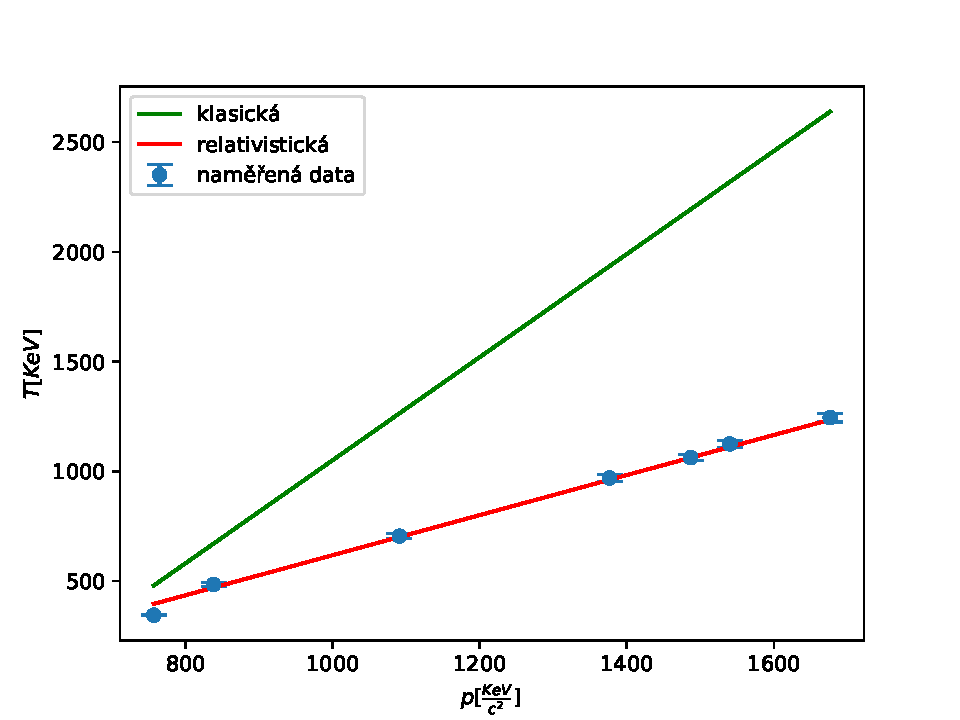
\includegraphics[scale=1]{figs/fig1.pdf}
  \caption{Závislosti $T(p)$ a $T_{r}(p)$}
  \label{gf:tp}
\end{figure}
\section{Diskuse}
Z grafu \ref{gf:tp} je vidět, že se naměřená data přibližují relativistické kinetické energii.
\section{Závěr}
Vytvořil jsem graf závislosti kinetické energie elektronu na jeho hybnosti.
\section{Zdroje}
\url{
  https://userswww.pd.infn.it/~moretto/fontana/project/software/2018/03/16/compton-edge.html
  }
\end{document}
